% document class and packages
\documentclass{beamer}
\usepackage{adjustbox}
\usepackage{algorithm,algorithmic}
\usepackage{amsmath}
\usepackage{amssymb}
\usepackage{color, colortbl}
\usepackage{graphicx}
\usepackage{hyperref}
\usepackage{pgfplots}
\pgfplotsset{compat=1.14}
\usepackage{tikz}

% indent for algorithm pseudo-code
\newlength\myindent
\setlength\myindent{1em}
\newcommand\bindent{%
  \begingroup
  \setlength{\itemindent}{\myindent}
  \addtolength{\algorithmicindent}{\myindent}
}
\newcommand\eindent{\endgroup}

% new commands and math operators
\newcommand*\conj[1]{\overline{#1}}
\newcommand{\iu}{{i\mkern1mu}}
\newcommand\abs[1]{\left|#1\right|}
\newcommand\norm[1]{\left\Vert#1\right\Vert}
\newcommand\diag[1]{\operatorname{diag}\left(#1\right)}
\newcommand\re[1]{\operatorname{Re}\left(#1\right)}
\newcommand\sv[2]{\operatorname{sv}_{#1}(#2)}
\newcommand\hd[2]{\operatorname{hd}(#1,#2)}
\newcommand\md[2]{\operatorname{md}(#1,#2)}
\newcommand\func[1]{\operatorname{function}~[#1]}
\DeclareMathOperator{\specr}{SpecR}
\DeclareMathOperator{\specdr}{SpecDR}
\DeclareMathOperator{\ipr}{IPR}

% 
\newtheorem{proposition}[theorem]{Proposition}

% remove figure caption prefix
\setbeamertemplate{caption}{\raggedright\insertcaption\par}

% hyperlinks setup
\hypersetup{colorlinks,breaklinks,
	urlcolor=[rgb]{0,0.75,1},
	linkcolor=[rgb]{0.75,0.75,0.75}}

% empty navigation symbols
\beamertemplatenavigationsymbolsempty

% remove navigation dots on miniframes
\makeatletter
\def\beamer@writeslidentry{\clearpage\beamer@notesactions}
\makeatother

% Use Theme
\usetheme{Warsaw}
\useoutertheme[footline=authortitle]{miniframes}
\useinnertheme[shadow=true]{rounded}

% Colors
\definecolor{black}{RGB}{0, 0, 0} % (primary, black)
\definecolor{lblue}{RGB}{102, 178, 255} % (secondary, light blue)
\definecolor{lgreen}{RGB}{102, 255, 178} %(tertiary, light green)
\definecolor{lsilver}{RGB}{224,224,224} % (text, light silver)
\definecolor{gray}{RGB}{128,128,128} % (graph node shade, gray)
\definecolor{white}{RGB}{255,255,255} % (graph node text, white)

% Beamer Colors
\setbeamercolor{palette primary}{bg=black,fg=lsilver}
\setbeamercolor{palette secondary}{bg=lblue,fg=lsilver}
\setbeamercolor{palette tertiary}{bg=black,fg=lsilver}
\setbeamercolor{structure}{fg=black} % itemize, enumerate, etc
\setbeamercolor{frametitle}{fg=black}

% Transparency for itemized listing
%\setbeamercovered{transparent}

% Title Page
\title{Round-Robin Rankability}
\author{Thomas R. Cameron}
\institute{Davidson College}
\date{June 18, 2019}

\begin{document}
% Title Frame
\begin{frame}
	\titlepage
\end{frame}

% Outline
%\AtBeginSection[]{
 %\frame<beamer>{
  %\frametitle{Outline}   
  %\tableofcontents[currentsection]
 %}
%}

%%%%%%%%%%%%%%%%%%%%%%%%%%%%%%%%%%%%%%%%%%%%%%%%%%%%%%
%								Algorithms
%%%%%%%%%%%%%%%%%%%%%%%%%%%%%%%%%%%%%%%%%%%%%%%%%%%%%%
\section{Algorithms}

\begin{frame}{Opening Remarks}
\begin{itemize}
\item	The spectral-degree characterization of perfect dominance graphs holds for all directed graphs with weights
	\[
	0\leq w_{ij}\leq 1.
	\]
	Therefore, we can weight ties with $1/2$.
\vfill
\item	There is an analogous characterization for perfect dominance graphs associated with double, triple, etc. round-robin tournaments.
	Therefore, we can naturally handle multiple games. 
\end{itemize}
\end{frame}

\begin{frame}{$\specr$ Algorithm}
For a single round-robin tournament we measure rankability using the following algorithm.
\vfill
\begin{algorithm}[H]
\caption{Spectral Rankability of for Round-Robin.}
\label{alg:specr}
\begin{algorithmic}
\STATE{$\func{r} = \specr\left(\Gamma\right):$}
\bindent
\STATE{$n\gets$ the number of vertices in $\Gamma$}
\STATE{$D\gets$ the out-degree matrix of $\Gamma$}
\STATE{$L\gets$ graph Laplacian of $\Gamma$}
\STATE{$S=\diag{n-1,n-2,\ldots,0}$}
\STATE{$r=1 - \frac{\hd{D}{S}+\hd{L}{S}}{2(n-1)}$}
\RETURN
\eindent
\end{algorithmic}
\end{algorithm}
\vfill
Note that this algorithm works for all digraphs with weights 
\[
0\leq w_{ij}\leq 1.
\]
\end{frame}

\begin{frame}{$\specdr$ Algorithm}
Four a double round-robin tournament we measure rankability using the following algorithm.
\vfill
\begin{algorithm}[H]
\caption{Spectral Rankability for Double Round-Robin.}
\label{alg:specdr}
\begin{algorithmic}
\STATE{$\func{r} = \specdr\left(\Gamma\right):$}
\bindent
\STATE{$n\gets$ the number of vertices in $\Gamma$}
\STATE{$D\gets$ the out-degree matrix of $\Gamma$}
\STATE{$L\gets$ graph Laplacian of $\Gamma$}
\STATE{$S=\diag{2(n-1),2(n-2),\ldots,0}$}
\STATE{$r=1 - \frac{\hd{D}{S}+\hd{L}{S}}{4(n-1)}$}
\RETURN
\eindent
\end{algorithmic}
\end{algorithm}
\vfill
Note that this algorithm works for all digraphs with weights 
\[
0\leq w_{ij}\leq 2.
\]
\end{frame}

%%%%%%%%%%%%%%%%%%%%%%%%%%%%%%%%%%%%%%%%%%%%%%%%%%%%%%
%								Sinquefield Cup
%%%%%%%%%%%%%%%%%%%%%%%%%%%%%%%%%%%%%%%%%%%%%%%%%%%%%%
\section{Sinquefield Cup}

\begin{frame}{Opening Remarks}
\begin{itemize}
\item	The Sinquefield Cup is an invite only round-robin chess tournament for Grand Master level players.
\vfill
\item	The Sinquefield Cup started in 2013 and the 2019 tournament takes place this August 16 - 29.
\vfill
\item	Throughout its history, the Sinquefield Cup has been one of the highest rated tournaments.
	For instance, in 2014, the average Elo rating was 2802, which is the highest average in the history of chess. 
\end{itemize}
\end{frame}

\begin{frame}{A Few More Details}
\begin{itemize}
\item	In 2013, the Sinquefield Cup was a double round-robin tournament comprised of 4 players.
\vfill
\item	In 2014, the Sinquefield Cup was a double round-robin tournament comprised of 6 players.
\vfill
\item	Since then, the Sinquefield Cup has been a single round-robin tournament comprised of 10 players. 
\end{itemize}
\end{frame}

\begin{frame}{Modeling Decisions}
Note that all weights $w_{ij}$ are initially set to zero.
Then, for each round we update as follows:
\vfill
\begin{itemize}
\item	If player $i$ beats player $j$, then $w_{ij}=w_{ij}+1$.
\vfill
\item	If player $j$ beats player $i$, then $w_{ji}=w_{ji}+1$.
\vfill
\item	If player $i$ and $j$ tie, then $w_{ij}=w_{ij}+1/2$ and $w_{ji}=w_{ji}+1/2$. 
\end{itemize}
\end{frame}

\begin{frame}{Round by Round Analysis}
\centering
\resizebox{0.8\textwidth}{!}{% Line Plot
\begin{tikzpicture}
	\begin{axis}[
		xlabel = Round Number,
		ylabel =  Rankability,
		legend pos = outer north east,
		cycle list name = color]
		\addplot coordinates{
			(1,0.1667)
			(2,0.3333)
			(3,0.4339)
			(4,0.5305)
			(5,0.6555)
			(6,0.7917)
		};
		\addplot coordinates{
			(1,0.1000)
			(2,0.2000)
			(3,0.3000)
			(4,0.4000)
			(5,0.5000)
			(6,0.6000)
			(7,0.7000)
			(8,0.7583)
			(9,0.7832)
			(10,0.7500)
		};
		\addplot coordinates{
			(1,0.1111)
			(2,0.2222)
			(3,0.2873)
			(4,0.3686)
			(5,0.4093)
			(6,0.4578)
			(7,0.5761)
			(8,0.6208)
			(9,0.6711)
		};
		\addplot coordinates{
			(1,0.1111)
			(2,0.1944)
			(3,0.2611)
			(4,0.3325)
			(5,0.4220)
			(6,0.4846)
			(7,0.5152)
			(8,0.5625)
			(9,0.6067)
		};
		\addplot coordinates{
			(1,0.1111)
			(2,0.1944)
			(3,0.2639)
			(4,0.3666)
			(5,0.4328)
			(6,0.4889)
			(7,0.5395)
			(8,0.5719)
			(9,0.6593)
		};
		\addplot coordinates{
			(1,0.1111)
			(2,0.1944)
			(3,0.2662)
			(4,0.3319)
			(5,0.3876)
			(6,0.4882)
			(7,0.5391)
			(8,0.5857)
			(9,0.6389)
		};
		\legend{Year 2013, Year 2014,Year 2015, Year 2016, Year 2017, Year 2018}
	\end{axis}
\end{tikzpicture}%
}
\end{frame}

\begin{frame}{Closing Remarks}
Note that the year 2013 has the highest rankability score after 6 rounds.
The scorecard for that year is shown below.
\vfill
\begin{figure}[H]
\centering
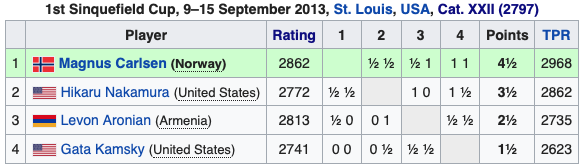
\includegraphics[width=0.75\textwidth]{figures/SinquefieldCup2013}
\end{figure}
\vfill
Note the uniform distribution of total points for each player, this seems very rankable to me!
\end{frame}

\begin{frame}{Closing Remarks}
The next most rankable year is 2014.
The scorecard for that year is shown below.
\vfill
\begin{figure}[H]
\centering
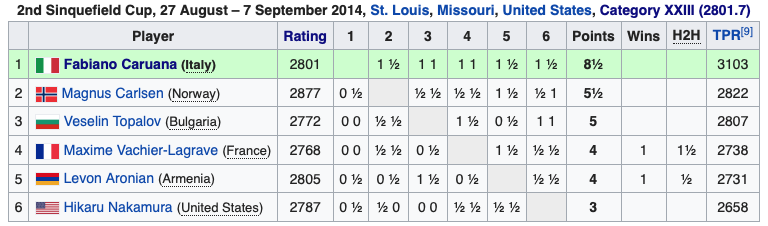
\includegraphics[width=0.75\textwidth]{figures/SinquefieldCup2014}
\end{figure}
\vfill
Note that this is the year that Fabiano went on his historical run.
However, there is a tie between 4 and 5 and not much difference between 2 and 3; hence, this year is slightly less rankable than 2013.
\end{frame}

\begin{frame}{Closing Remarks}
The least rankable years were 2016 and 2018. 
Both scorecards are shown below.
\vfill
\begin{figure}[H]
\centering
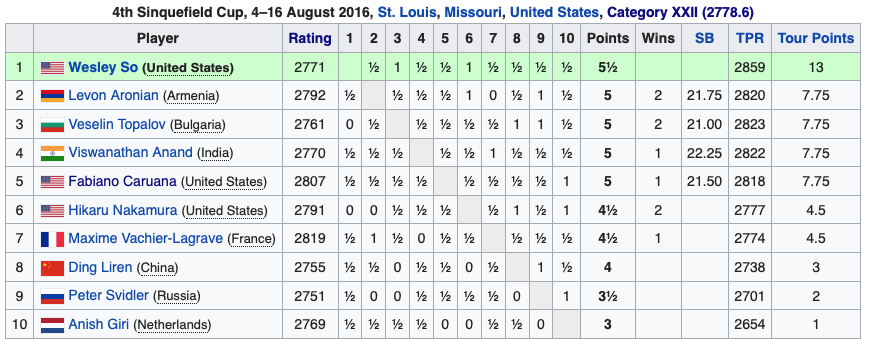
\includegraphics[width=0.75\textwidth]{figures/SinquefieldCup2016} \\
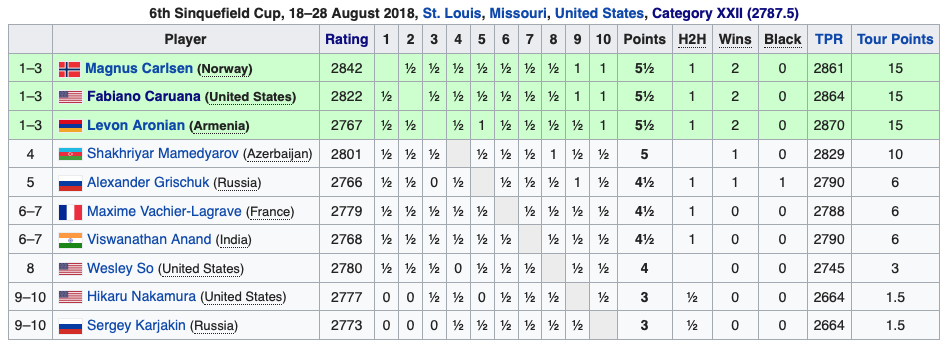
\includegraphics[width=0.75\textwidth]{figures/SinquefieldCup2018}
\end{figure}
\end{frame}

\begin{frame}{Closing Remarks}
Note that there is a 4 way tie for second place in 2016.
Furthermore, each place is only separated by half a point.
Similarly, in 2018 there was a 3 way tie for first place. 
Interestingly, the winners agreed to split the prize and not deal with elimination games.
Certainly, these years are less rankable than 2013 and 2014. 
\end{frame}

%%%%%%%%%%%%%%%%%%%%%%%%%%%%%%%%%%%%%%%%%%%%%%%%%%%%%%
%								Next Steps
%%%%%%%%%%%%%%%%%%%%%%%%%%%%%%%%%%%%%%%%%%%%%%%%%%%%%%
\section{Next Steps}

\begin{frame}{What's Next?}
\begin{itemize}
\item	Now that the spectral rankability can deal with multiple games, I would like college basketball conference data where the modeling decision is similar to the one chosen here.
\vfill
\item	We can also deal with ties, so I would like college sports data (conferences only) where ties are allowed. I think baseball allows for ties?
\vfill
\item	I would also like to do "week by week" analysis like was done here (round by round).
	This should be easy with college football.
	Can we do other sports?
\vfill
\item	I am still on the lookout for dominance data from animal populations, or plurality voting data.
	Perhaps we should talk to an expert?
\end{itemize}
\end{frame}

\end{document}